\documentclass{ba-kecs}
\usepackage{graphicx,, url}
\usepackage[numbers]{natbib}
\usepackage{amssymb,amsmath}

\title{Turtlebot SLAM }

\author{Maurice Hermans, Lukas Kang, Michael Norget, Thomas Nowicki, Oliver Trinnes}

\begin{document}

\maketitle

\begin{abstract}
Robots are used for a lot of tasks nowadays, to perform an assignment a robot needs a map of the environment. Using external referencing methods, like GPS, they can locate them self. Sometimes the maps are provided, making the task easier to perform. It becomes far more difficult when the robot has no map or external reference available. The task of mapping an environment can be split into two main components, namely exploration and SLAM which stands for Simultaneous Localization And Mapping. The exploration determines the path the robot takes to explore the unknown space of the environment. Exploration is based on the idea of frontiers, these are cells which separate unexplored cells from free explored cells. The exploration strategy then determines the next location the robot should move to. The SLAM part incorporates the new data as is becomes available when the robot moves to unexplored areas and takes measurements of previously unrecorded space. One intuitive way is to represent all the data as a graph where the nodes represent a pose of the robot and the edges connecting two nodes the measured constraints. The algorithm then tries to find a configuration of nodes which is maximally consistent with the constraints. This article will describe an implementation of this so called GraphSLAM with frontier exploration. All the implemented code is first tested and validated in a simulator and later run on a real robot, a TurtleBot.

This article accompanies the research project "TurtleBot SLAM" from the Master "Artificial Intelligence" of Maastricht University.
\end{abstract}

\section{Introduction}
\label{sec:intro}
Nowadays mobile robots succeed to assist industry and society in a diverse set of problems. Transportation, search, rescue and, more specifically, automated vacuum cleaning are examples from different fields. Typically, mobile robots can move through an environment using legs or wheels. In addition they are able to gather information about their surrounding using sensors. Some even have devices similar to the human arm or hand which allows them to interact with the environment. The vacuum cleaning robot depicted in Figure \ref{fig:vacuum_cleaner} is an example of a robot which has wheels to move around. Furthermore it is equipped with a set of sensors. These sensors provide data about the location of obstacles as well as, for example, gaps in the floor the robot is moving on. To efficiently perform this task robots needs a map of its environment. For some tasks map data is available for the robot from the beginning. Provided a map the robot can locate itself using the incoming sensor data or, if available, GPS data. For tasks in unknown environments, however, the robot must make its own map of the environment.

The acquisition of these maps has been a major research focus in the robotics community \cite{ Grisetti, Montemerlo02, Montemerlo, Thrun}. Building or learning these maps under position uncertainty provided only sensor measurements is often referred to as the Simultaneous Localization And Mapping (SLAM) problem. A large variety of solutions is available to it.
\begin{figure}[h]
	\centering
		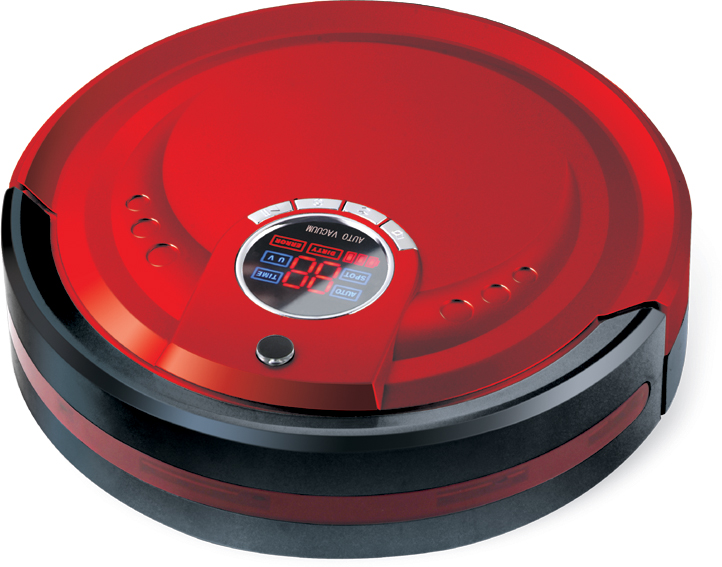
\includegraphics[width=0.50\textwidth]{figures/vacuum_cleaner.jpg}
	\caption{A vacuum cleaner robot \citep{VacuumRobot}.}
	\label{fig:vacuum_cleaner}
\end{figure}

The remainder of this paper is structured as follows. Section \ref{sec:sota} provides the state of the art of the discussed fields. Section \ref{sec:impl} is about the implementation details of the methods used. Section \ref{sec:exp} explains the experiments ran to validate and benchmark the implemented methods and also evaluate the obtained results. Section \ref{sec:disc} discusses the acquired results of the experiments and proposes future research based on those. And the last section wraps up the paper with the conclusions of this research.

Subsection \ref{sec:problem} defines the problem statement for this project.
\subsection{Problem Statement}
\label{sec:problem}
This paper accompanies a university group project. The project assignment is to implement both a graph-based SLAM algorithm and an autonomous exploration strategy. The hardware to be used is a mobile robot called TurtleBot. Thus the final product should allow the robot to autonomously navigate through an unknown environment and simultaneously build a map of it using a Graph SLAM.

Information about the programming environment, the TurtleBot, autonomous exploration and SLAM methods are given in Section \ref{sec:sota}.  

\section{State of the art}
This section presents the state of the art of the hardware, software, and methods used for this project. Subsection \ref{subsec:ros} gives an outline about the operating system in which the product is implemented. Next, Subsection \ref{subsec:turtle} is about the TurtleBot. At last, autonomous exploration (Subsection \ref{subsec:sotaExplore}) and SLAM (Subsection \ref{subsec:sotaSlam}) 
\label{sec:sota} are defined and explained.
\subsection{ROS}
\label{subsec:ros}
The Robot Operating System (ROS) \cite{Quigley} is the environment used throughout the development of all product components for this project. As described by Quigley et al., writing software for robots is difficult since there is a large variety of possible hardware set-ups. This also makes code reuse non-trivial. An additional problem is the amount of code needed to actually ``run" something on a robot. A deep stack including driver-level software, perception modules and, for example, abstract reasoning systems is required before the actual problem can be attacked. Since the necessary expertise and effort is beyond capabilities of most single researchers, an environment that features this functionality is required to achieve anything similar to the problem specified in Subsection \ref{sec:problem}.

To deal with the above mentioned problems robotics researchers have created a wide variety of frameworks. Many robotic software systems are currently used by researchers and industry \cite{Kramer}. Each of these frameworks is designed for a specific purpose, though. Generally, none of these systems is directly applicable to a problem it was not designed for in the first place.

The ROS framework used in this paper is the product of trade-offs and prioritizations. The emphasis of this framework lies on large-scale integrative robotics research, making it useful in a wide variety of situations. The difference between ROS and the above mentioned frameworks, is ROS' applicability to a wide range of hardware set-ups. It provides several so called stacks. Each is an assembly of code made to solve one specific problem. To run a stack or your own code on any robot it is necessary to configure the robot and the ROS framework in a way that they can communicate with each other. For most robots the configuration is straight forward thanks to the on-line documentation of ROS \citep{Roswiki}.  An example for a stack is the multi-robot simulation environment ``Stage". It is explained in the following paragraph.

\subsubsection{ROS' simulator: ``Stage"}
During the development process of a system running on a robot one crucial part is testing. A ROS stack called Stage enables the developers to test code on a simulated robot. Stage allows the simulated robot to move around in virtual environments. It visualizes sensor data and other robot data when required. The user can load her own maps into stage and specify the kind of noise to be applied to measurements. A second important stack needed especially for validation is RViz. It visualizes all requested data. In Figure \ref{fig:stage_and_rviz} Stage and RViz are presented next to each other. While Stage (Left) shows the real map, RViz (Right) presents the map data as seen by the robot.

\subsection{TurtleBot}
\label{subsec:turtle}
The product of this project is designed to run on a mobile robot called TurtleBot (Figure \ref{fig:turtlebot}) \citep{turtlebot}. It is a low-cost, customizable, personal robot kit. The base of the TurtleBot is an iRobot Create (A). It holds a battery pack and a 150 degrees/second Single Axis Gyro. The model shown in Figure \ref{fig:turtlebot} uses a Microsoft Kinect sensor (B), the one used in this paper uses a laser range sensor and a laptop (C) to run all the processes. The robot can also be customized using the mounting hardware (D). The robot runs on an open-source SDK based on ROS which integrates all the software needed to get the TurtleBot running. Some capabilities are included in ROS and can be used in the TurtleBot after minor configurations. These include mapping and navigation, for example. 
\begin{figure}[h]
	\centering
		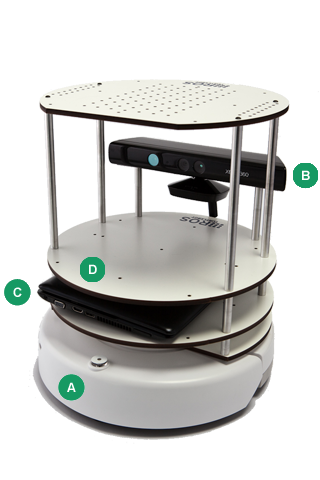
\includegraphics[width=0.50\textwidth]{figures/turtlebot.png}
	\caption{A TurtleBot}
	\label{fig:turtlebot}
\end{figure}

\subsection{Exploration}
\label{subsec:sotaExplore}
Usually robots localize themselves and navigate through environments using a map which is provided by an external source. In this case navigating from one location to another is an easy problem. If the robot does not have access to a map, navigating through an environment is problematic. The problem treated in this paper (Subsection \ref{sec:problem}) assumes an unknown environment and, hence, no map. The robot needs to be able to explore its environment without any knowledge about it. It needs to rely on the incoming laser and odometry data only. In addition to the creation of the map and the localization of itself (the SLAM problem) the robot needs to explore the environment as efficient as possible. We define a good exploration strategy as one that generates an accurate map in the shortest amount of time.

Ideally the robot updates its internal map of the environment constantly while moving. One idea to efficiently explore the world is to move to locations which maximize the robot's information gain. This target location needs to be extracted from the limited information the robot has collected with its sensors.
To achieve this the robot makes use of the idea of frontier-based exploration, first introduced by Yamauchi \cite{Yamauchi} in 1998. Frontiers are defined to be the boundaries between free and unexplored space. Intuitively, when a robot moves to a frontier it is likely that it makes measurements in previously unexplored space. Given that new data can be added to its map. The explored region grows once the robot reaches a frontier. Moreover an extended map results in new frontiers. By constantly moving to frontiers the robot expands its knowledge about the environment.

\subsection{SLAM}
\label{subsec:sotaSlam}
As mentioned in Section \ref{sec:intro} Simultaneous Localization And Mapping (SLAM) is the process of building a map based on sensor data while simultaneously localizing yourself in an unknown environment.

Other approaches estimate the complete trajectory from the set of measurements. These approaches address the so called full SLAM problem and they typically rely on least-square error minimization techniques \cite{Leastsquares}.

An intuitive way to formulate the SLAM problem is to consider it as a pose graph optimization problem. The nodes of the graph represent robot poses or landmarks. The edges encode sensor measurements that constraint the connected poses. Once such a graph is constructed the graph-based SLAM, or Graph SLAM, method tries to find a configuration of the nodes that is maximally consistent with the constraints contained in the edges.\\

SLAM is a problem because localization requires a map and mapping requires the location of the device or robot that wants to create a map. There are quite a few approaches that successfully solve the SLAM problem. 
In general there are two interpretations it. The first estimates the current robot pose along with the map. The core of such a system is a filtering technique. New measurements augment and refine the estimate as they become available. Due to their incremental nature these filtering approaches are commonly referred to as on-line SLAM methods. FastSlam \citep{Montemerlo02} is an example of an on-line SLAM implementation. It uses a Particle Filter to approximate the robots pose and the landmark positions on the map. Other methods have the goal to find the trajectory of the robot and the map. These solve the full SLAM problem and typically rely on least-square error minimization techniques \cite{Leastsquares} to find adequate estimates.  
An example of such a an approach is graph-based SLAM or Graph SLAM.

\subsubsection{Graph SLAM}
An intuitive way to formulate the SLAM problem is to view it as a pose graph optimization problem. Each pose along the trajectory of the robot is represented by one node. Edges are labeled with relative spatial information between the connecting nodes. This graph is built incrementally. While the robot is in motion, new nodes are added to the graph. Building up the graph, as explained above, is a straight forward procedure. The essence of the Graph SLAM method, however, is the optimization step. In this step the algorithm tries to find a spatial configuration of the trajectory which is maximally consistent with a system of constraints obtained from the edges. This problem is commonly solved using least-square error minimization techniques \citep{Grisetti}.

\section{Implementation}
\label{sec:impl}

The software explained in this section are implemented in the object-oriented programming language C++. The code is specifically designed for the ROS environment (see Subsection \ref{subsec:ros}). The installation process for ROS, as performed for this paper, can be reviewed on \cite{swarmlab}.

\subsection{Program structure}
An overview of the relevant components of the final software product is given in Figure \ref{fig:program_structure}. The top two boxes represent the implemented packages. The left one performs the Graph SLAM algorithm (Subsection \ref{sec:implSLAM}), including the initialization and optimization of the pose graph and the correction by scan matching (Subsection \ref{sec:scan}). It also creates a map of the explored environment by maintaining an occupancy grid (Subsection \ref{sec:mapping}). The right package is responsible for autonomous exploration (Subsection \ref{sec:wfd}). This includes an algorithm for efficiently navigating through unknown space to gather as much information about the environment as possible.

\begin{figure}[htbp]
	\centering
		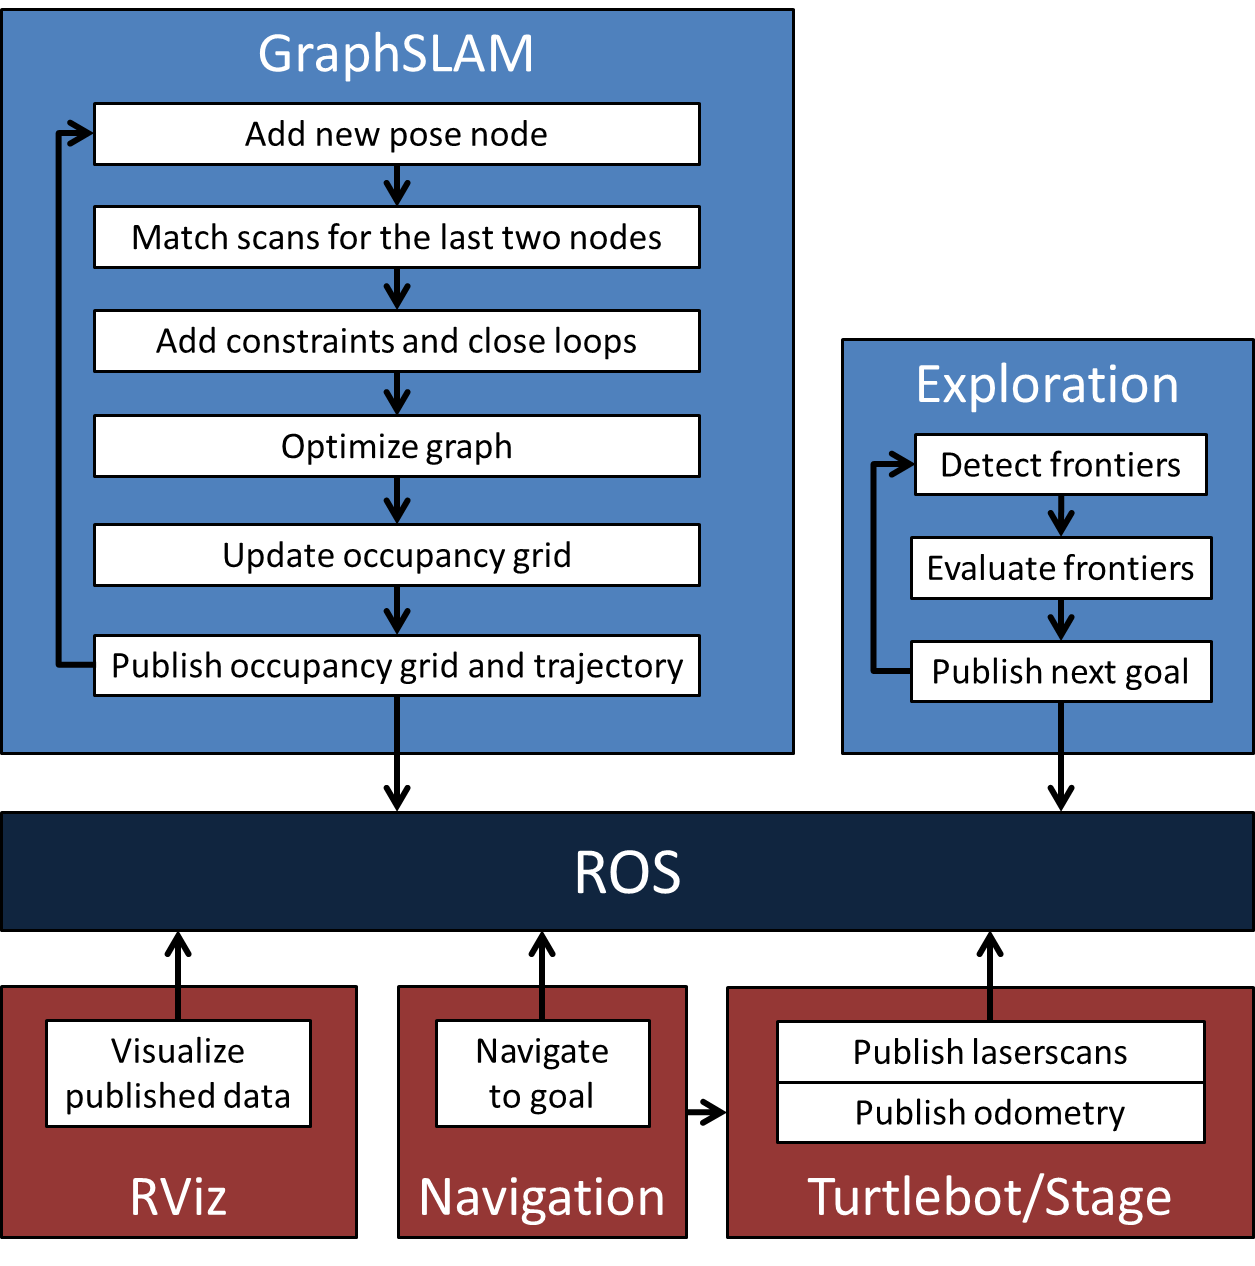
\includegraphics[width=0.45\textwidth]{figures/Program_structure.png}
	\caption{Overview of the structure and functionalities of the relevant software components}
	\label{fig:program_structure}
\end{figure}

Both packages publish data to the shared environment of ROS. This data is then used by the other packages to create an interdependent but modular program structure.

The implemented packages are making use of the external library ``Eigen" \citep{eigen}. It provides extensive linear algebra operations. Included are simple matrix operations as well as advanced techniques. Two techniques which are used in this project are Singular Value Decomposition and sparse Cholesky factorization.


\subsection{Graph SLAM}
\label{sec:implSLAM}
The implemented Graph SLAM algorithm is based on \citep{Grisetti}. The graph consists of nodes representing poses along the robot trajectory. Odometry and sensor measurements are incorporated into the constraints contained in the edges. Similar to the Graph SLAM procedure explained in Section \ref{subsec:sotaSlam}, an edge connects two adjacent poses of the robot. 
\begin{figure}[h]
	\centering
		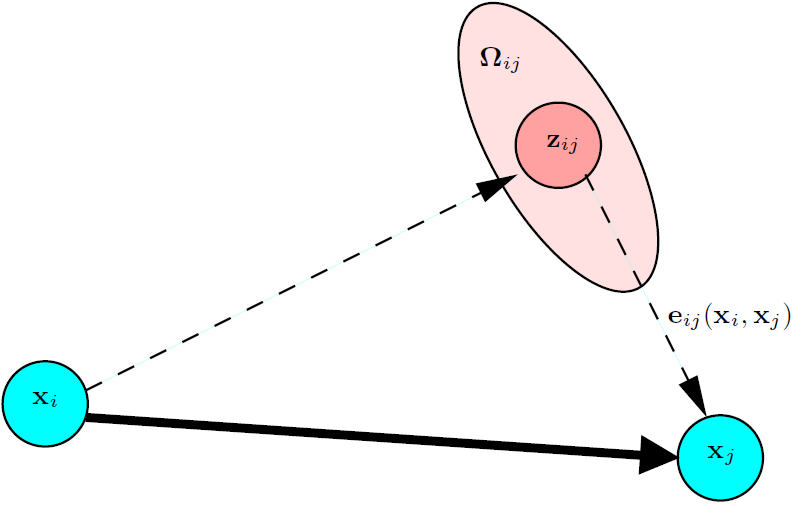
\includegraphics[width=0.50\textwidth]{figures/graph.png}
	\caption{An example of a simple graph (based on \citep{Grisetti}).}
	\label{fig:turtlebotexample_graph}
\end{figure}
When the graph is created the pose graph is optimized according to the constraints. This ``optimized" trajectory then determines the positions of obstacles on the map. The laser scan data are refined according to the poses they were obtained at. Each edge, thus, is labeled with the spatial difference between two poses \(x_i\) and \(x_j\). Let this error be denoted by \(e_{ij}(x_i, x_j)\). This information is obtained from a combination of odometry data and laser range sensor data. In fact, the raw odometry data is corrected using a laser scan matcher (see Subsection \ref{sec:scan}). 
Figure \ref{fig:turtlebotexample_graph} shows a sketch of a graph created by the algorithm. Two poses \(x_i\) and \(x_j\) are connected by an edge (Solid arrow). The ellipse at the top illustrates the label of the edge.

This graph-based SLAM approach calculates the most likely path as follows:
First it finds the Jacobians \(A\) and \(B\) of every two estimated poses connected by an edge.
\begin{equation}
\label{eq:jacobi_a}
	A_{ij} = \frac{\partial e_{ij}(x)}{\partial x_i}
\end{equation}
\begin{equation}
\label{eq:jacobi_b}
	B_{ij} = \frac{\partial e_{ij}(x)}{\partial x_j}
\end{equation}
Note that in Equations \ref{eq:jacobi_a} and \ref{eq:jacobi_b} the x represents the current guess of the concerning robot pose. As explained above, \(e_{ij}(x_i, x_j)\) is the error between the two poses \(x_i\) and \(x_j\). The Jacobians \(A\) and \(B\) are then added to a matrix \(H\) (Equation \ref{eq:H}).
\begin{equation}
\label{eq:H}
\begin{aligned}
	H_{[ii]} += A^{T}_{ij} \Omega_{ij} A_{ij} \\
	H_{[ij]} += A^{T}_{ij} \Omega_{ij} B_{ij} \\
	H_{[ji]} += B^{T}_{ij} \Omega_{ij} A_{ij} \\
	H_{[jj]} += B^{T}_{ij} \Omega_{ij} B_{ij} \\
\end{aligned}
\end{equation}
In this equation $\Omega_{ij}$ is the information matrix of a measurement between \(x_i\) and \(x_j\). It is defined as shown in Equation \ref{eq:omega}.
Sigma is the $3 \times 3$ covariance matrix of the measurements. In our implementation the diagonal of $\Sigma$ is filled with arbitrary values.
\begin{equation}
\label{eq:omega}
\Omega = \Sigma^{-1}
\end{equation}
In addition to the matrix $H$ a coefficient vector \(b\) is kept up to date as shown in Equation \ref{eq:b}. This vector together with the \(H\) form a set of linear constraints.
\begin{equation}
\label{eq:b}
\begin{aligned}
	b_{[i]} += A^{T}_{ij} \Omega_{ij} e_{ij} \\
	b_{[j]} += B^{T}_{ij} \Omega_{ij} e_{ij} 
\end{aligned}
\end{equation}
The optimization of the vector \(x = (x_1, ..., x_n)^T \) according to the constraints specified in \(H\) and \(b\) is the core of this approach. This step is performed using sparse Cholesky factorization. 

A new node is added to the graph once the robot moves 0.5 meters. The algorithm optimizes the trajectory like explained once a new node is added.\\
In one special case the algorithm adds an extra edge, connecting to non-adjacent nodes, to the graph. This happens when the distance between the two connected robot poses is smaller than a margin. In fact, this special case enables the algorithm to create loops in the graph and more accurately estimate the robots trajectory and the map. This procedure is referred to as ``loop closing" (see Subsection \ref{sec:loopClosing}). 
\subsection{Scan matching}
\label{sec:scan}
The scan matcher, used by this program, is necessary to acquire an optimized movement vector between two robot poses. This is needed by the Graph SLAM algorithm (see Subsection \ref{sec:implSLAM}). The scan-matcher realized for this project can be divided into two steps. At the beginning, the two scans are matched making use of raw odometry data, retrieved by the robot's motion sensor. This is improved upon by running an iteration of the iterative closest point algorithm (ICP). It tries to align the two scans minimizing the total distance of each point in the first scan to its nearest neighbor in the second. 

The general procedure of the algorithm is to first find the nearest neighboring point in the second scan for all point in the first. To achieve this nearest neighbor search is used.
In this implementation multiple points can have the same corresponding neighbor-point. If there is no point from the other scan within a specified radius of one point, it is excluded. These outliers would influence further calculations negatively.
The next step in the process is to calculate the centroids of both clouds. These are subtracted from every point in the concerning cloud. In that way the clouds are centered at the origin. The calculated points are then added to two separate $2 \times n$ matrices, where $n$ is the number of neighbor pairs. Next the rotation matrix which transforms one cloud to the other is needed. The Singular Value Decomposition (SVD) of the product of the two previously mentioned matrices returns three new matrices $U$, $\Sigma$ and $V$. The required rotation matrix R can be obtained as described in Equation \ref{eq:RVUT}.
\begin{equation}
\label{eq:RVUT}
 R = V * U^T
\end{equation}
The translation vector $t$ is the difference between the two centroids. $R$ and $t$ together form a rigid transformation. This transformation matches the two scans. Moreover it is used to correct the robot's odometry data.

\subsection{Mapping}
\label{sec:mapping}
The map is internally represented as an occupancy grid. It consists of cells which hold information about obstacles, free/- and unknown space. 

The occupancy grid is a structure that is represented by a one-dimensional array. The size of an occupancy grid has to be tuned problem specific. A too large grid can lead to performance problems. If the grid is too small, however, the map will be inaccurate. Fitting a map on a smaller grid results in a low resolution.
Internally the program represents the grid as a two dimensional array. This makes navigating to either side more intuitive. Each grid cell contains an integer value. The value-range for ROS' occupancy grid lies between $-1$ and $100$ \cite{occupancy}. The values indicate the state as follows:
\begin{description}
\item{$-1$} : Unknown space, not yet covered by robot's perception sensors
\item{$0$} : Known free space, robot can drive on it safely
\item{$1-100$} : Probability of being an obstacle, $1$ being a low probability and $100$ being a definite obstacle.
\end{description}
\begin{figure}[htbp]
	\centering
		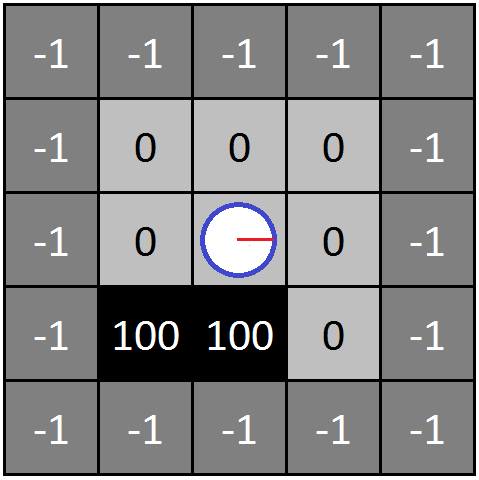
\includegraphics[width=0.45\textwidth]{figures/Occup.png}
	\caption{A visualized occupancy grid}
	\label{fig:Occupancy}
\end{figure}
Figure \ref{fig:Occupancy} shows an example occupancy grid. The robot stands in the center of it and makes one measurement consisting of several laser scans. Each scan returns the range it was able to reach. The returned range is either the maximally possible range of the laser or a lower value, indicating an obstacle (value of 100). The range is transformed into global coordinates with respect to the robot's location, orientation and the bearing of the laser beam. The resulting point is then transferred into the occupancy grid as an obstacle if the maximum range was not reached. The cells lying in a straight line between the transformed range and the robot are considered free space (value of 0), since the laser was able to pass through this area. All the cells that are not affected by any of the previous steps remain unexplored (value of -1). Naturally, this is the case for cells behind obstacles, out of range and directly behind the robot.

As time progresses, the robot explores more of its environment. As explained above, the locations of the observed obstacles need to be extracted from the laser-scan data. The program keeps track of the scan-data for every robot pose saved in the trajectory \(x = (x_1, ..., x_n)^T \). Since the laser-scan data is relative to the pose of recording, new information is added to the map once the robot's trajectory is adjusted by the Graph SLAM module. When a new scan is made, it is added to the occupancy grid after the trajectory has been updated. When a loop closure is detected, the complete occupancy grid is updated. All previous scan points are refined relative to their corresponding recording poses and the grid is regenerated.

\subsection{Exploration}
\label{sec:wfd}
One part of the assignment is autonomous exploration. The robot has to drive autonomously through an unknown world. This feature is implemented using Wavefront frontier detection (WFD).

WFD is a frontier-based exploration algorithm \citep{Keidar}. It uses four different data structures. These store map and frontier information during the search process. They are:
\begin{enumerate}
\item{Map-Open-List}
\item{Map-Close-List}
\item{Frontier-Open-List}
\item{Frontier-Close-List}
\end{enumerate}
To understand the need of these four structures it is necessary to know that WFD is using a breadth first search (BFS), starting at the current robot position. Moreover frontier detection requires the robot to have an internal representation of the current environment. In this implementation an occupancy grid (Subsection \ref{sec:mapping}) is used.
Upon launching the algorithm it first searches for unoccupied space around the current robot location. These grid cells are saved in the Map-Open-List. 
Frontiers are found by making use of the occupancy grid's structure. The criterion for a map-point to be a frontier is the existence of both, unknown space and known unoccupied space, in adjacent map-points. When a frontier point is found a new BFS is performed. Starting at the current point it extracts all adjacent frontier points and connects them to one frontier. It is saved in the Frontier-Open-List. The benefit of using WFD is that by maintaining these lists, the algorithm only needs to incorporate points that have not been iterated yet. In fact, the algorithm keeps track of detected open space and frontiers using the above mentioned list. Following iterations make use of this information because they do not need to consider previously known regions any more.
 
Exploration does not only consist of finding frontiers. Based on the frontiers a target location for the robot needs to be selected. Navigating to the closest frontier points is the simplest frontier-based exploration strategy. For this project, however, a more sophisticated implementation is chosen. Instead of sending the robot to the closest frontier point, a small search is performed to find suitable destinations. Generally, a small region around each frontier cell is searched. The goal is to give each frontier point a rating on how well it is suited as a destination. For this purposes an evaluation function has been implemented. It incorporates three features that are used to evaluate goals to be sent to the navigation stack. They are :
\begin{enumerate}
\item{Number of obstacles in the area}
\item{Distance to the previous goal}
\item{Distance between frontier and robot location}
\end{enumerate}
The first two features have a weight one, whereas the third is assigned a weight of five. This configuration turned out to create the best results (see Subsection \ref{sec:navEval}) The weighted sum of the features is used to find the goal to be sent to the navigation stack. This evaluation function enables the algorithm to select a reachable destination for the robot in almost every case. The frontier cells are sent to the move\_base in the order of the rating. When the navigation stack fails to steer the robot to a designated goal within a time constraint, the next best goal replaces the previous. The information gain is still next to optimal since the selected goal is preferred to be close to frontier points. At last the second feature makes sure that the robots path is smooth. Selecting a goal near the previous one makes the robot avoid too many loops in the emerging graph.

\section{Experiments and results}
\label{sec:exp}
This section presents the results of the TurtleBot SLAM implementation as described in Section \ref{sec:impl}. Several outputs of the visualization tool RViz are presented and discussed. Comparisons are drawn between different variations of the implementation. Finally, the performance of the program is evaluated.

\subsection{Visualization}
\label{sec:visual}
When running the program, RViz and Stage are started. Stage shows the robot in its actual position on an accurate test map (see Figure \ref{fig:stage_and_rviz} left). RViz visualizes the current belief of the robot about its environment, position and trajectory (see figure \ref{fig:stage_and_rviz} right).

The components of the pose graph and the environment are highlighted by the following labels:

\begin{description}
\item[Green dots:]Past poses of the robot, saved as nodes of the pose graph
\item[Red arrows:]Past orientations of the robot, included in the nodes of the pose graph
\item[Blue lines:]Measurement constraints between the connected poses
\item[Yellow dots:]Frontier points detected by the Wavefront frontier detection algorithm
\item[Orange dot:]Next navigation goal
\item[Black area:]Detected obstacles
\item[Light gray area:]Detected free space
\item[Dark gray area:]Unexplored space
\end{description}

\begin{figure}[htbp]
	\centering
		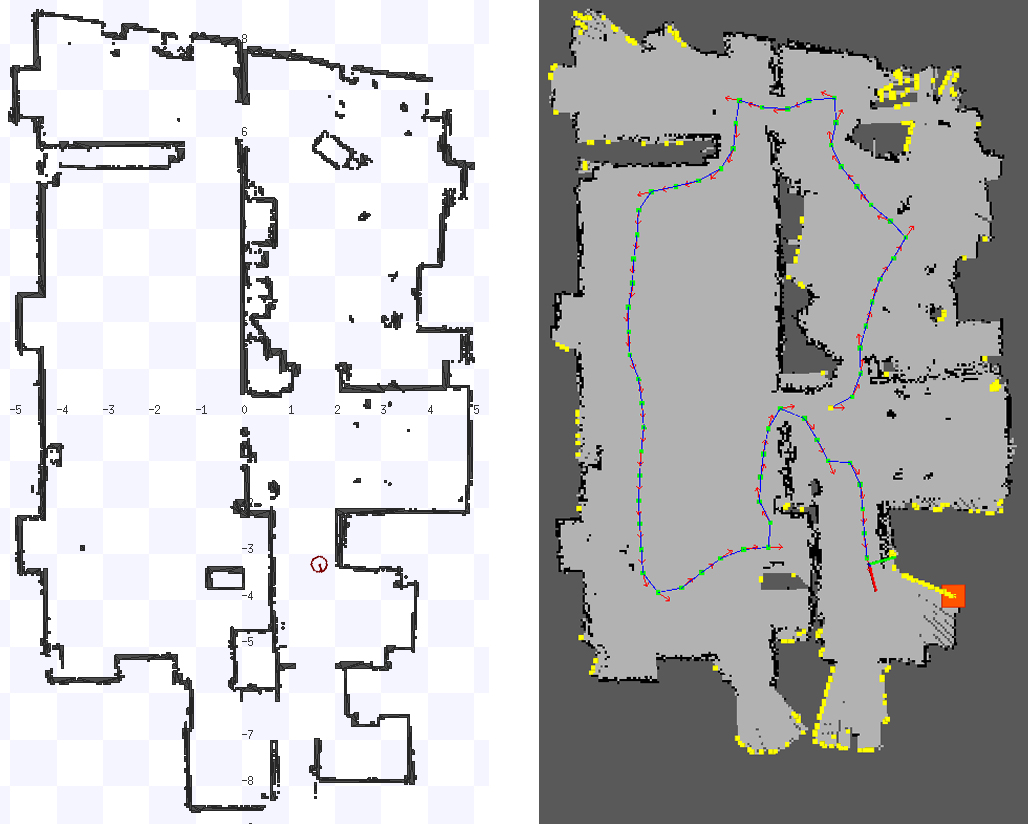
\includegraphics[width=0.50\textwidth]{figures/Stage_and_rviz.jpg}
	\caption{Robot and environment visualization with Stage (Left) and RViz (Right).}
	\label{fig:stage_and_rviz}
\end{figure}

\subsection{Loop closing effect}
\label{sec:loopClosing}
One of the core properties of the Graph SLAM algorithm is the correction of the pose graph and the map whenever a loop closing is detected. This means that when the robot has been exploring an unknown area and then re-enters an explored area, the transformation between the current pose and the past, re-detected, pose gives essential information about the complete pose graph. It corrects the current belief about environment and position.

The effect of loop closing detection is illustrated in Figure \ref{fig:loop_closing_comparison}. The transparent red lines indicate the real map data, while the underlying black areas indicate the belief of the robot about obstacles in the environment.

The left part of Figure \ref{fig:loop_closing_comparison} shows the explored map when walking an eight-shaped path through the map without applying loop detection. The belief about the map differs from the actual map in many areas. Especially in the lower half the map is inaccurate. This is because this half has been explored last, exposing it to most of the measurement uncertainties.

The right part of Figure \ref{fig:loop_closing_comparison} depicts the exploration when following the same path as before. This time loop closing is enabled during the process of exploration. The outcome is a pose graph with seven additional constrains in comparison to the previous experiment. More constraints provide more information for correcting the poses and corresponding measurements. One can now see that the lower half of the belief about the map is much more accurate, since the area in the center has been re-detected by the algorithm.

\begin{figure}[htbp]
	\centering
		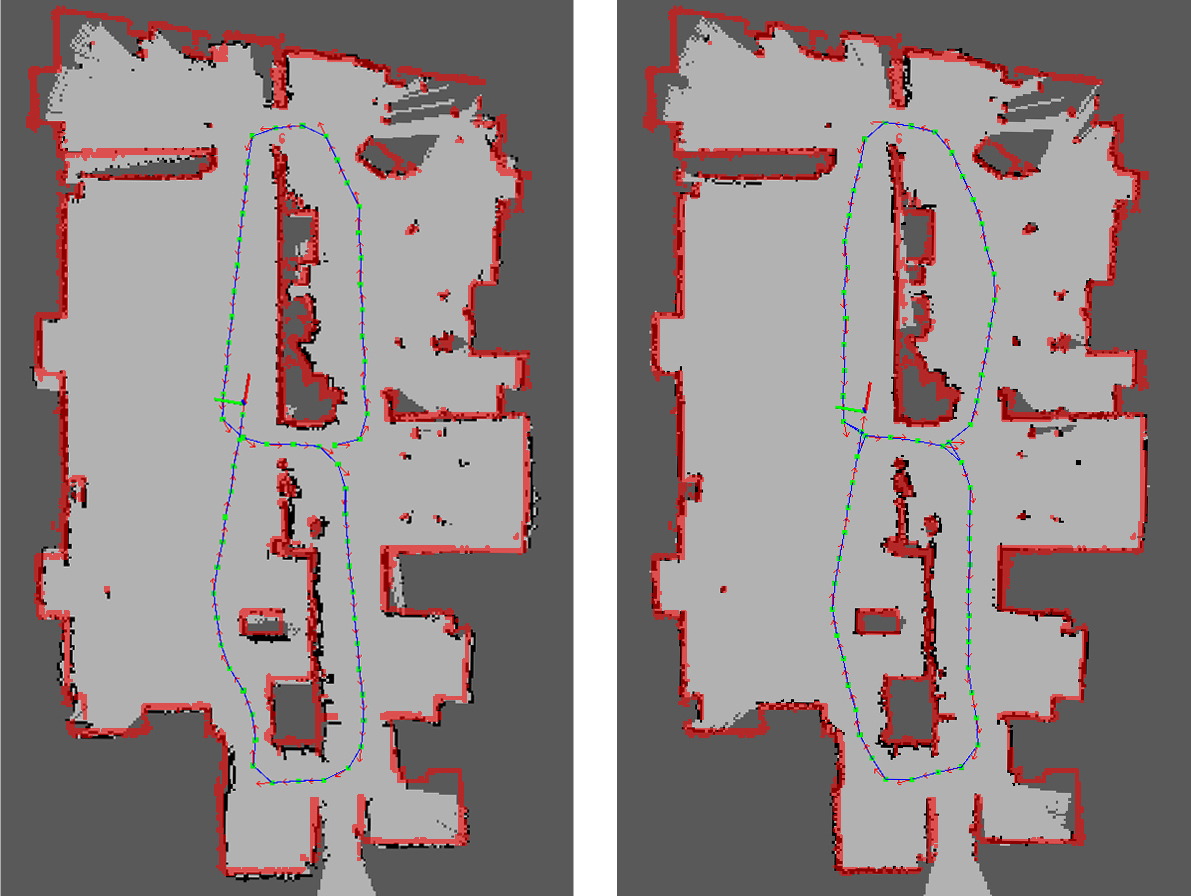
\includegraphics[width=0.50\textwidth]{figures/Loop_closing_compared.jpg}
	\caption{Observed environment without (left) and with (right) loop closing of the pose graph}
	\label{fig:loop_closing_comparison}
\end{figure}
The next section explains which experiments have been conducted in order to find an optimal exploration strategy. It presents results for different goal selection methods.

\subsection{Navigation evaluation}
\label{sec:navEval}
An important aspect which has a high impact on the exploration behavior of the robot is the strategy by which the next navigation goal is determined. When facing the decision for the next goal, the robot needs to rely on the information it has access to. Frontiers can be spread all over the current map. The most obvious first implementation idea is to select the frontier which lies closest to the robot as the next navigation goal. This is desirable because the time the robot needs to reach the goal is low. In addition the robot gathers new information when the frontier point is reached.

Figure \ref{fig:navigation_comparison} shows three resulting exploration paths of the robot as well as the explored maps after 300 seconds. In Figure \ref{fig:navigation_comparison}(a) the simple strategy, as explained above, was applied. 10 nodes and 14 constraints have been created in the pose graph. Compared to other tests this is very little information. Also the nodes are limited to a small area of the map. Applying the simple strategy results in a low degree of exploration. This is due to the fact that when only considering the closest frontier point there is a high risk that points are selected which are very close to obstacles. When the navigation stack tries to find a path to this point, it inflates the obstacles first. This causes goals which are very close to any kind of obstacle to be unreachable. When a point has been discovered to be unreachable, the next closest point to the robot is chosen. This, however, is likely to be unreachable as well.

In order to overcome the above explained problems another exploration strategy is considered. Obstacles have to be taken into account to be able to select reachable points as the next goal. In this new strategy obstacles within a radius of 50 grid cells of the frontier point are counted. This number is added to the distance between the robot and the concerning frontier point. The point with the smallest sum is selected as the next goal. The application of this strategy is shown in figure \ref{fig:navigation_comparison}(b). The robot managed to explore the map within 300 seconds, creating a pose graph containing 104 nodes and 150 constraints. However, one can see that the robot did not take a very exploration-efficient route through the map. There are a lot of unreasonable turns in areas that are already explored, while unexplored areas are omitted for the time being.

To avoid counter-intuitive routes another aspect is to be added to the evaluation of every frontier point. The distance between the currently evaluated point and the previous navigation goal. When this distance is minimized in addition to the previous evaluation features, the algorithm will select the next goals in a chain-like fashion. This creates an intuitive exploration path through the map (Figure \ref{fig:navigation_comparison}(c)). The robot was able to explore the map within only 150 seconds, creating a much smaller pose graph of 64 nodes and 66 constraints. This evaluation feature has been given a weight factor of $5$ to increase the effect on the goal selection.

\begin{figure}[htbp]
	\centering
		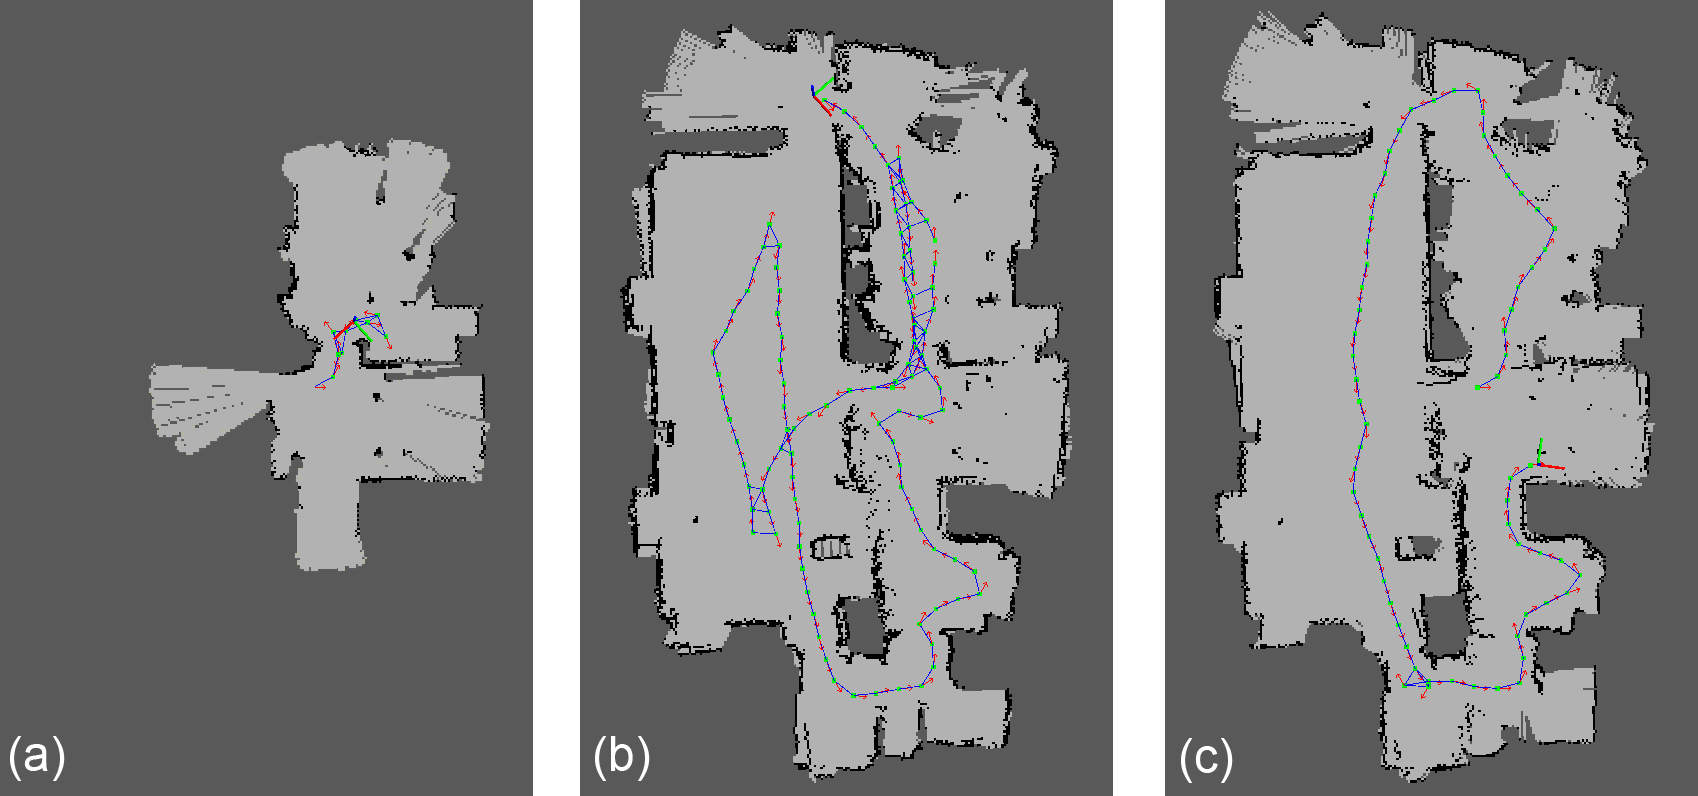
\includegraphics[width=0.50\textwidth]{figures/Navigation_comparison.jpg}
	\caption{Resulting robot trajectory when applying different strategies for selecting the next navigation goal}
	\label{fig:navigation_comparison}
\end{figure}

\subsection{Runtime analysis}
\label{sec:runtime}
The implemented Graph SLAM algorithm has been tested on its feasibility. Navigating the robot manually, the complete test map has been explored, building up a pose graph of 123 nodes and 150 constraints. While doing so, the runtime of the complete update-function was measured in microseconds. This function is executed whenever a new node is added to the graph. It contains the algorithms for scan matching and Graph SLAM correction, which have also been assessed separately.

Figure \ref{fig:runtime} shows the outcome of this runtime measurement. Naturally the runtime increases with increasing graph size, especially due to the growing matrices in the Graph SLAM algorithm.

\begin{figure}[htbp]
	\centering
		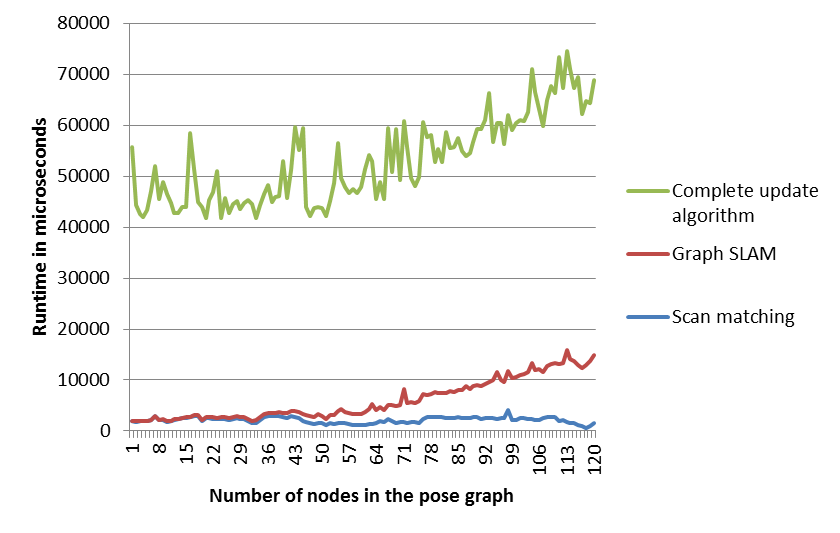
\includegraphics[width=0.50\textwidth]{figures/Runtime.png}
	\caption{Runtime of the Graph SLAM update function in micro seconds}
	\label{fig:runtime}
\end{figure}

Even with a graph size of more than 100 nodes, the runtime of the function stays in a feasible range between 60 and 80 milliseconds. The robot can be moved without delay. Taking only the Graph SLAM update into account, the runtime even stays below 20 milliseconds. In contrast the scan matching is executed outstandingly quickly since it is independent of the size of the pose graph. Most of the time is occupied by updating the occupancy grid because every single grid cell has to be redrawn for every pose. In order to compromise this, the update of the complete occupancy grid is only executed every three seconds and only if a loop closing is detected.

\section{Discussion}
\label{sec:disc}
In this section the results of the implemented methods are evaluated and discussed. 
Subsection \ref{disc:expl} deals with the exploration strategy. Subsection \ref{disc:grSlam} presents the evolution of the Graph SLAM implementation. Different stages of it are evaluated.
\subsection{Exploration strategy}
\label{disc:expl}
The Wavefront Frontier detection algorithm \citep{Keidar} succeeds in finding frontiers in a fast and accurate manner (see Subsection \ref{sec:visual}). It turned out, however, that finding the frontiers is only part of autonomous exploration. Subsections \ref{sec:wfd} and \ref{sec:visual} explain the various possibilities there are for selecting a feasible goal for the robot. Adding features to the evaluation of possible destinations showed to make selection more successful. During the process of implementation this evaluation function evolved to a prosperous and accurate goal chooser.
\\
\subsection{Graph SLAM}
\label{disc:grSlam}
Developing a feasible Graph SLAM algorithm showed to be a challenging task. In earlier stages of the project another Graph SLAM algorithm was implemented.
It is based on \cite{Thrun}. 
Nodes are created for each odometry measurement as well as for every map feature detected by the robot. All occupancy grid cells containing an obstacle are considered map features. This is necessary because all information for the occupancy-grid map is inherited in these features. The output of this implementation is a vector containing the positions of the landmarks as well as the trajectory of the robot. Here the constraints labeling the edges are created using Jacobians similar to the final approach (see Subsection \ref{sec:implSLAM}). The major difference lies in the node creation. Here, additional nodes are added for landmarks while the previous implementation considered the robot's trajectory only. An additional difference lies in the fact that this implementation uses features to characterize the map. The algorithm needs to compare every feature from the new scan has to the ones detected earlier. This ``correspondence test" has to be performed and repeated along with the complete optimization procedure until convergence. 

While testing it turned out that the algorithm's time complexity is too high for real time observations. Even with a reduced number of laser beams the map update takes an infeasible amount of time after a few steps only. 
\begin{table}[h]
\begin{center}
\scalebox{1}{
\begin{tabular}{|l||c|c|c|l}
\hline
\# steps & 2 beams & 10 beams & 30 beams\\
\hline \hline
2	& 1 ms & 2 ms	&  22 ms	\\
4	& 2	ms & 11 ms	&  269 ms	\\
6	& 3 ms & 24 ms	&  1069 ms	\\
8	& 4 ms & 56 ms	&  2682 ms	\\
10	& 5 ms & 126 ms	&  5250 ms	\\
12	& 6 ms & 273 ms	&  9170 ms	\\
14	& 7 ms & 485 ms	&  15895 ms	\\
\hline
\end{tabular}
}
\end{center}
\caption{The time the Graph SLAM implementation proposed by \citep{Thrun} needed using the specified number of laser beams after the specified number of steps.}
\label{tab:graphResults}
\end{table}
Note that the number of beams used for the other implementation greatly exceeds the ones in Table \ref{tab:graphResults}. While the working Graph SLAM method deals with roughly 390 laser beams, this one has major difficulties with not more than 30.
This points out that this implementation is unable to create a map in reasonable time.

Implementing the algorithm suggested in \citep{Grisetti} (Subsection \ref{sec:implSLAM}) showed to be well suited for attacking the problem statement of this project. The maps created by the algorithm are accurate (see Subsection \ref{sec:visual}). The difference between the output map and the real map is negligible (see Figure \ref{fig:loop_closing_comparison}). Maps are created in real time and loop closures are added when needed. In fact, the algorithm is able to keep updating the map with no noticeable delay (see Section \ref{sec:exp}). Even when the robot is controlled by the exploration module and navigated by ROS' move\_base package the program runs smoothly.

The next subsection suggests a few ideas about how this research could be continued. In doing so proposes are made for each part of this project.

\subsection{Future research}
As mentioned in Section \ref{disc:expl} the exploration strategy evolved during the process of testing. This does not mean that it cannot be improved upon. More features like, for instance, loop closings can be taken into account. This would lead to more constraints to be added to the graph. More constraints could then result in an even more accurate assessment of the robot trajectory. This new feature would require to be tuned well, since more constraints also lead to higher space and time complexities. 
\\

The Graph SLAM algorithm proposed by \citep{Grisetti} can be improved as well. Considering the suggested change in the exploration algorithm, the method would need to cope with a larger number of edges and nodes.
The current implementation uses sparse Cholesky factorization to find the most optimal spatial configuration of the trajectory. This method is inherited in the ``Eigen" library \ref{sec:impl}. Although sparse Cholesky factorization solves the linear system in an efficient manner, it is likely that even better algorithms emerge in the future. Since the time complexity of the Graph SLAM method depends almost entirely on the technique used, new methods would directly improve upon the running time of the algorithm.

The deprecated Graph SLAM implementation clearly has most room for improvement. The TurtleBot used for this research project has to rely on laser and odometry data only. Extracting features from laser data is out of scope of this project. Doing so could dramatically improve the performance of the method, though. 
A robot equipped with for instance a color sensor is much more suited to successfully perform this Graph SLAM method. Colored objects could serve as landmarks and large parts of the feature detection could be left out. Implementing a powerful feature-extractor for laser data is definitely a possible solution. Applying the method to a robot that provides different kinds of data is the preferred one, nevertheless.

The last section draws a conclusion based on the results (Section \ref{sec:exp}) and the discussion (Section \ref{sec:disc}).
\section{Conclusion}
\label{sec:conc}
In conclusion Graph SLAM is an algorithm with a variety of implementations. Incorporating the map into the graph showed to lead to an infeasible time complexity (Section \ref{sec:disc}). The Graph SLAM method as described by Grisetti et al. \citep{Grisetti} is able to solve the full SLAM problem in real time (Subsection \ref{sec:runtime}). The created maps are accurate (Subsection \ref{sec:navEval}). Furthermore WFD succeeds in quickly detecting frontiers (Subsection \ref{sec:runtime} and Figure \ref{fig:runtime}). It turned out that the exploration strategy, besides frontier detection, is a crucial task. The developed evaluation function accurately assesses suitable goal locations (Subsection \ref{disc:expl}). It allows the robot to drive smooth, intuitive paths (Figure \ref{fig:navigation_comparison}). The program containing these components solves the problem specified in Subsection \ref{sec:problem}.

\bibliography{references}
\nocite{*}
\onecolumn
\appendix

\end{document}
